%!TEX root = main.tex

\chapter{Implementation}
In this chapter we describe how we implemented the project, and maybe how we did some tests on it for results. 
Section \ref{sec:integration} how we integrated bwapi with lida
Section \ref{sec:detectors} feature detectors we made
Section \ref{sec:actionexecution} how action are executed from lida to bwapi



\section{Integration}
\label{sec:integration}
The LIDA framework is written in Java, so to use with with BWAPI we have to use the java implementation of BWAPI, JNIBWAPI. JNIBWAPI is a java interface that talks with BWAPI using a shared memory bridge. But to use the LIDA framework this has to be integrated with JNIBWAPI. So to accomplish this we implement the domain specific modules of the LIDA framework to make calls to JNIBWAPI. 


\begin{figure}[h!tb]
\centering
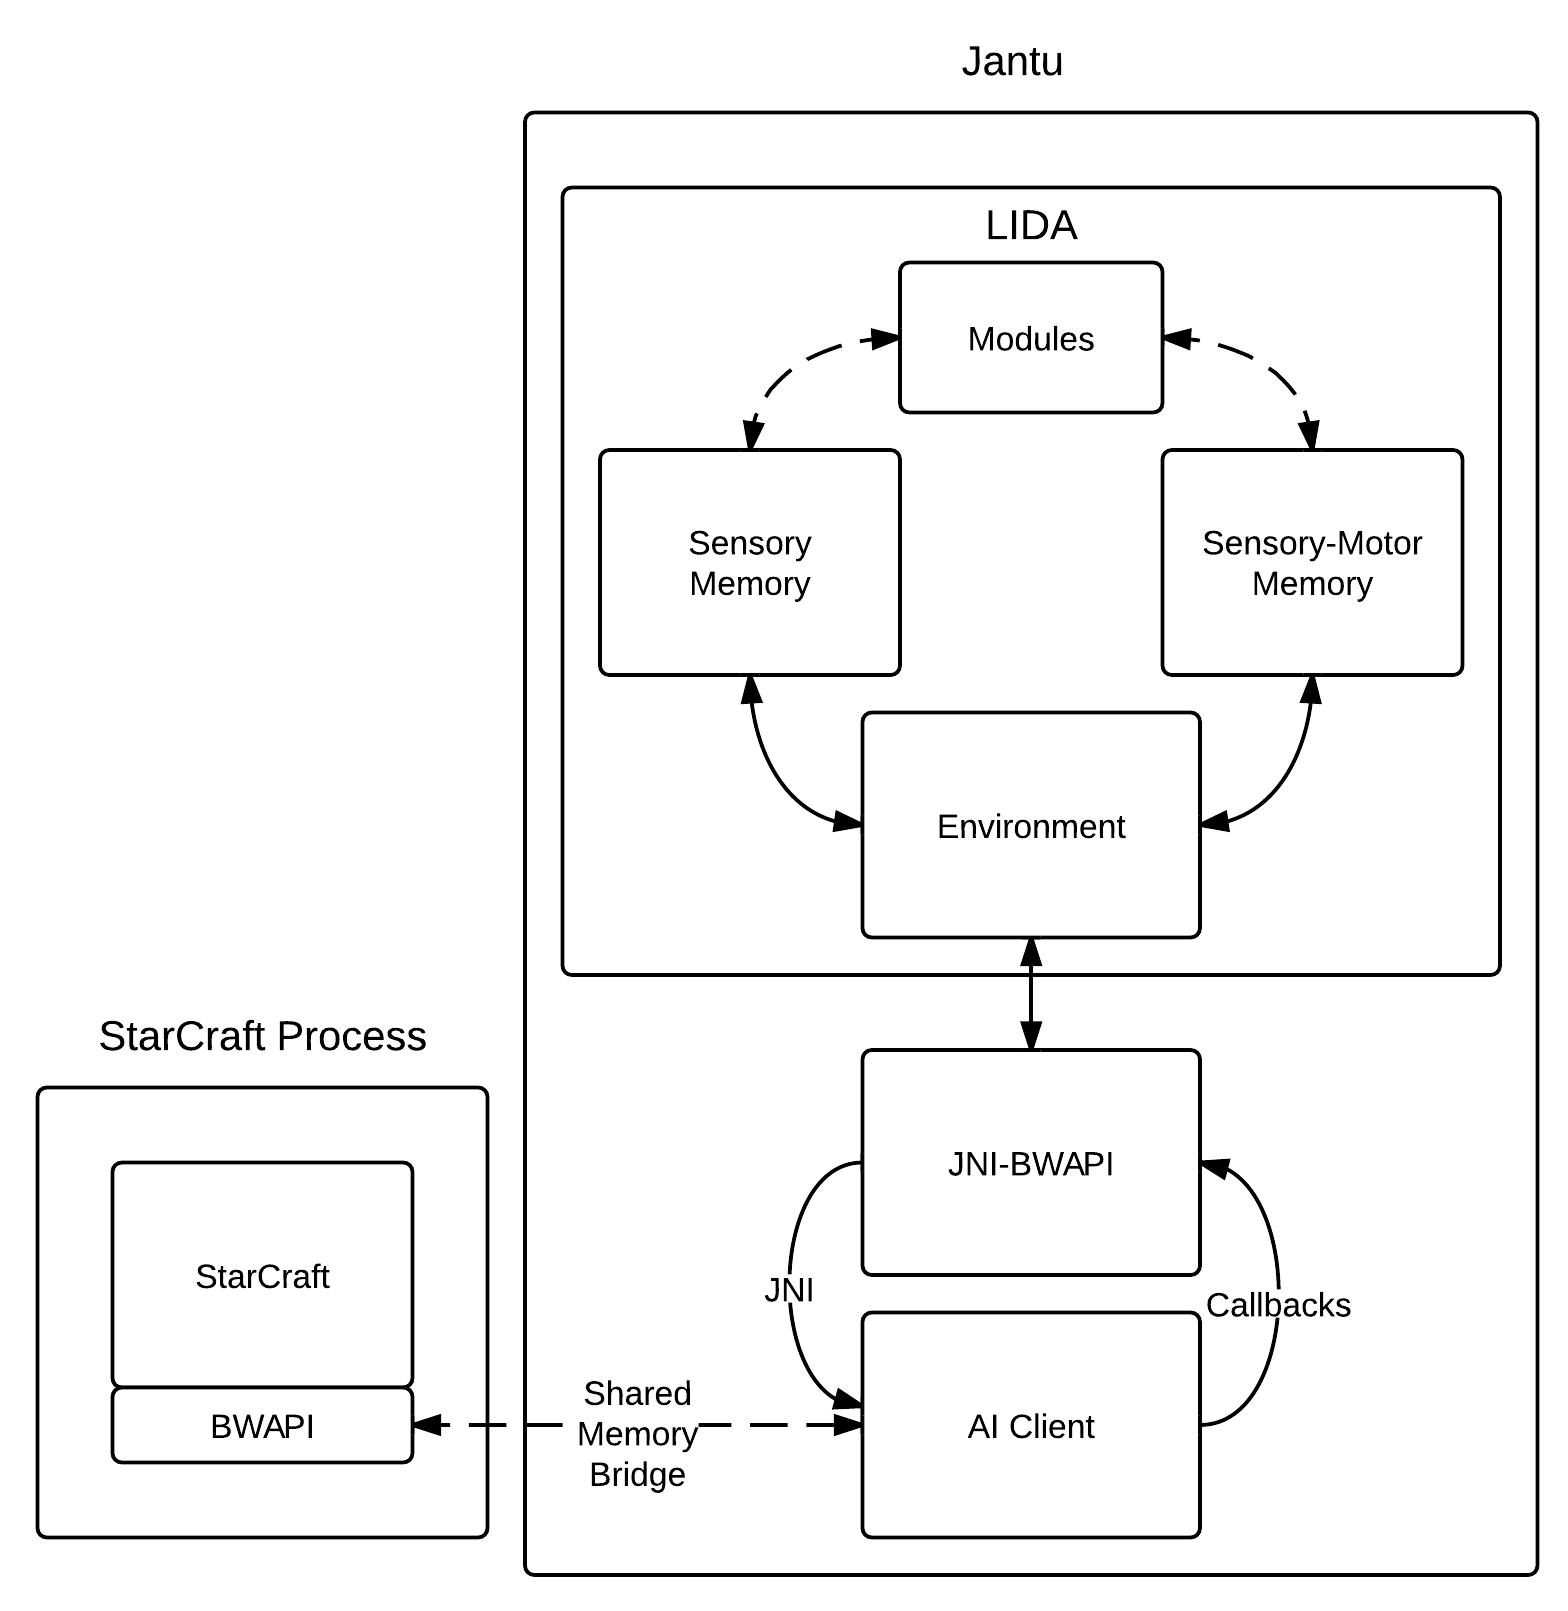
\includegraphics[scale=1.0]{graphics/jantu.png}
\caption{A general architecture overview of Jantu}
\label{fig:jantu}
\end{figure}

Figure \ref{fig:jantu} shows a general overview of the Jantu bots architecture, which consists of 3 main parts. In the Starcraft process the game it self runs together with BWAPI injected into the game client. Since this is all running in c++ and we are using the Java interface for BWAPI our code is run in a separate process that communicates with the Starcraft process using a shared memory bridge, this enables JNI-BWAPI to make calls to BWAPI and retrieve information back across the bridge. 

In the Jantu process JNI-BWAPI is running together with the LIDA framework. 

%si noe om at vi oppdaterte jni bwapi? og hva gjorde vi egentlig

In order to integrate the LIDA framework with JNI-BWAPI we setup the framework first with the configurations we needed to get it up and running. This involves describing and structuring the modules you need in different XML configuration files. Also in these files we configure what kind of information that will be possible to use and transmit internally in the LIDA framework. 

JNI-BWAPI consists of different models and types that represent Starcraft information like units and buildings together with a lot of native functions that can be called to communicate with BWAPI. So we integraded this with LIDA by using a custom implementation of the Environment class in LIDA. This class becomes the interface between the domain specific modules of LIDA, the sensory memory and sensory-action memory, and JNI-BWAPI. 

\section{Detectors}
\label{sec:detectors}
Feature detectors is how LIDA perceives it's environment and identifies important aspects of the current game state. They are task that are run at specific intervals and parses the game state at that time in order to identify a given feature that can later be used in different modules in LIDA recognize thoughts and concepts. 

\section{Action Execution}
\label{sec:actionexecution}
Action are executed with commands!
